\chapter{Methode}
In dit hoofdstuk wordt het ontwerp en de realisatie van de pipet besproken, evenals de gemaakte keuzes.

\section{Conceptueel ontwerp}
\subsection{Literatuurstudie}
De literatuurstudie bestaat uit patenten zoals\ \cite{RN16} en\ \cite{RN17} die analoge pipetten beschrijven. Deze patenten tonen aan dat deze pipetten een eenvoudige zuigerwerking gebruiken, wat belangrijk is voor het ontwerp. Patenten zoals\ \cite{RN35},\ \cite{RN36}, en\ \cite{RN38} tonen aan dat een stappermotor gebruikt kan worden voor de zuigerwerking met hoge precisie.

\section{Hardware ontwerp}
Dit gedeelte behandelt de hardwarekeuzes. De onderdelen werden ontworpen in Autodesk Inventor en geprint met Prusa Mk3S en Mk4 printers.

\subsection{Muurelementen}
Er werd gekozen voor modulaire elementen, wat toekomstige aanpassingen mogelijk maakt. De muren zijn geprint in PLA, wat gezien de lage structurele eisen voldoende is. In latere iteraties werden de muren lichter door de vlakken te verwijderen. De muurelementen zijn geparametriseerd voor verschillende hoogtes. Het 80mm-element voorziet ruimte voor de zuiger, en het 30mm-element voor de askoppeling.

\subsection{Bodemplaat en geleidestaven}
De muurelementen en geleidestaven worden op de bodemplaat gemonteerd. De bodemplaat heeft gaten voor de geleidestaven en andere onderdelen zoals de eindeloopschakelaar en spuit. De tegengedraaide moeren zorgen voor extra stevigheid en bevestigen de ge-3D-printte elementen.

\subsection{Tussenplaat en motorplaat}
De tussenplaat scheidt de askoppeling en de zuigerkamer. De motorplaat heeft ruimte voor de Nema 8 stappermotor, die met M2-schroeven wordt bevestigd.

\subsection{Loodschroef, motor en askoppeling}
De T4-loodschroef heeft een spoed en lood van 1mm. De motor is een Nema 8 stappermotor (0.4N-cm koppel) die krachtig genoeg is om de zuiger aan te drijven. De flexibele askoppeling compenseert voor kleine misaligneringen door het 3D-printen.

\subsection{Geleideslede}
De geleideslede bestuurt de zuiger en is versterkt met hoge wanden om oscillaties te verminderen. De zuiger wordt vastgeklemd met een twee-delige klem die vervangbaar is afhankelijk van de zuigermaat.

\subsection{Zuiger}
Er is gekozen voor standaard verkrijgbare 1000$\mu$l-spuiten (DB ISO 7886--1 Luer Slip 1ml) om luchtdichte problemen te voorkomen. Deze spuiten kunnen eenvoudig vervangen worden.

\section{Elektronica ontwerp}
\subsection{Componentenlijst}
\begin{table}[H] 
    \begin{tabular}{l|c|c} 
        \textbf{Component} & \textbf{Type} & \textbf{Aantal} \\
        Motor & Nema 8 (8HS15--0604D) & 1 \\
        Motor driver & BigTreeTech TMC2209 & 1 \\
        Microcontroller & ESP32-WROOM-32 & 1 \\
        Eindeloopschakelaar & Micro Limit switch & 1 \\
        5V Voeding & Vrij te kiezen\footnotemark & 1 \\
    \end{tabular} 
    \caption{Componentenlijst.}\label{tab:componentenlijst} 
\end{table}

\subsection{Motor}
De gekozen Nema 8 motor heeft een koppel van 0.4N-cm, voldoende om de zuiger te verplaatsen. De motor wordt gestuurd in een open lus en moet regelmatig naar de nulpositie worden gebracht met een eindeloopschakelaar.

\subsection{Driver}
De TMC2209 stappermotor driver gebruikt de ``StealthChop''-technologie, wat zorgt voor stillere en soepelere motorwerking met hogere precisie.

\subsection{Microcontroller}
De ESP32-WROOM-32 is gekozen voor zijn hoge kloksnelheid, wat zorgt voor een snelle respons bij het sturen van stap-signalen naar de motor.

\subsection{Aansluiting}
De elektronische componenten zijn aangesloten zoals te zien in \autoref{fig:schematische_aansluiting}, met de motor verbonden aan de TMC2209 driver en de ESP32. De voeding is 5V, en de ESP32 vereist een voeding tussen 3.3V en 5V.

\begin{figure}[H] 
    \centering 
    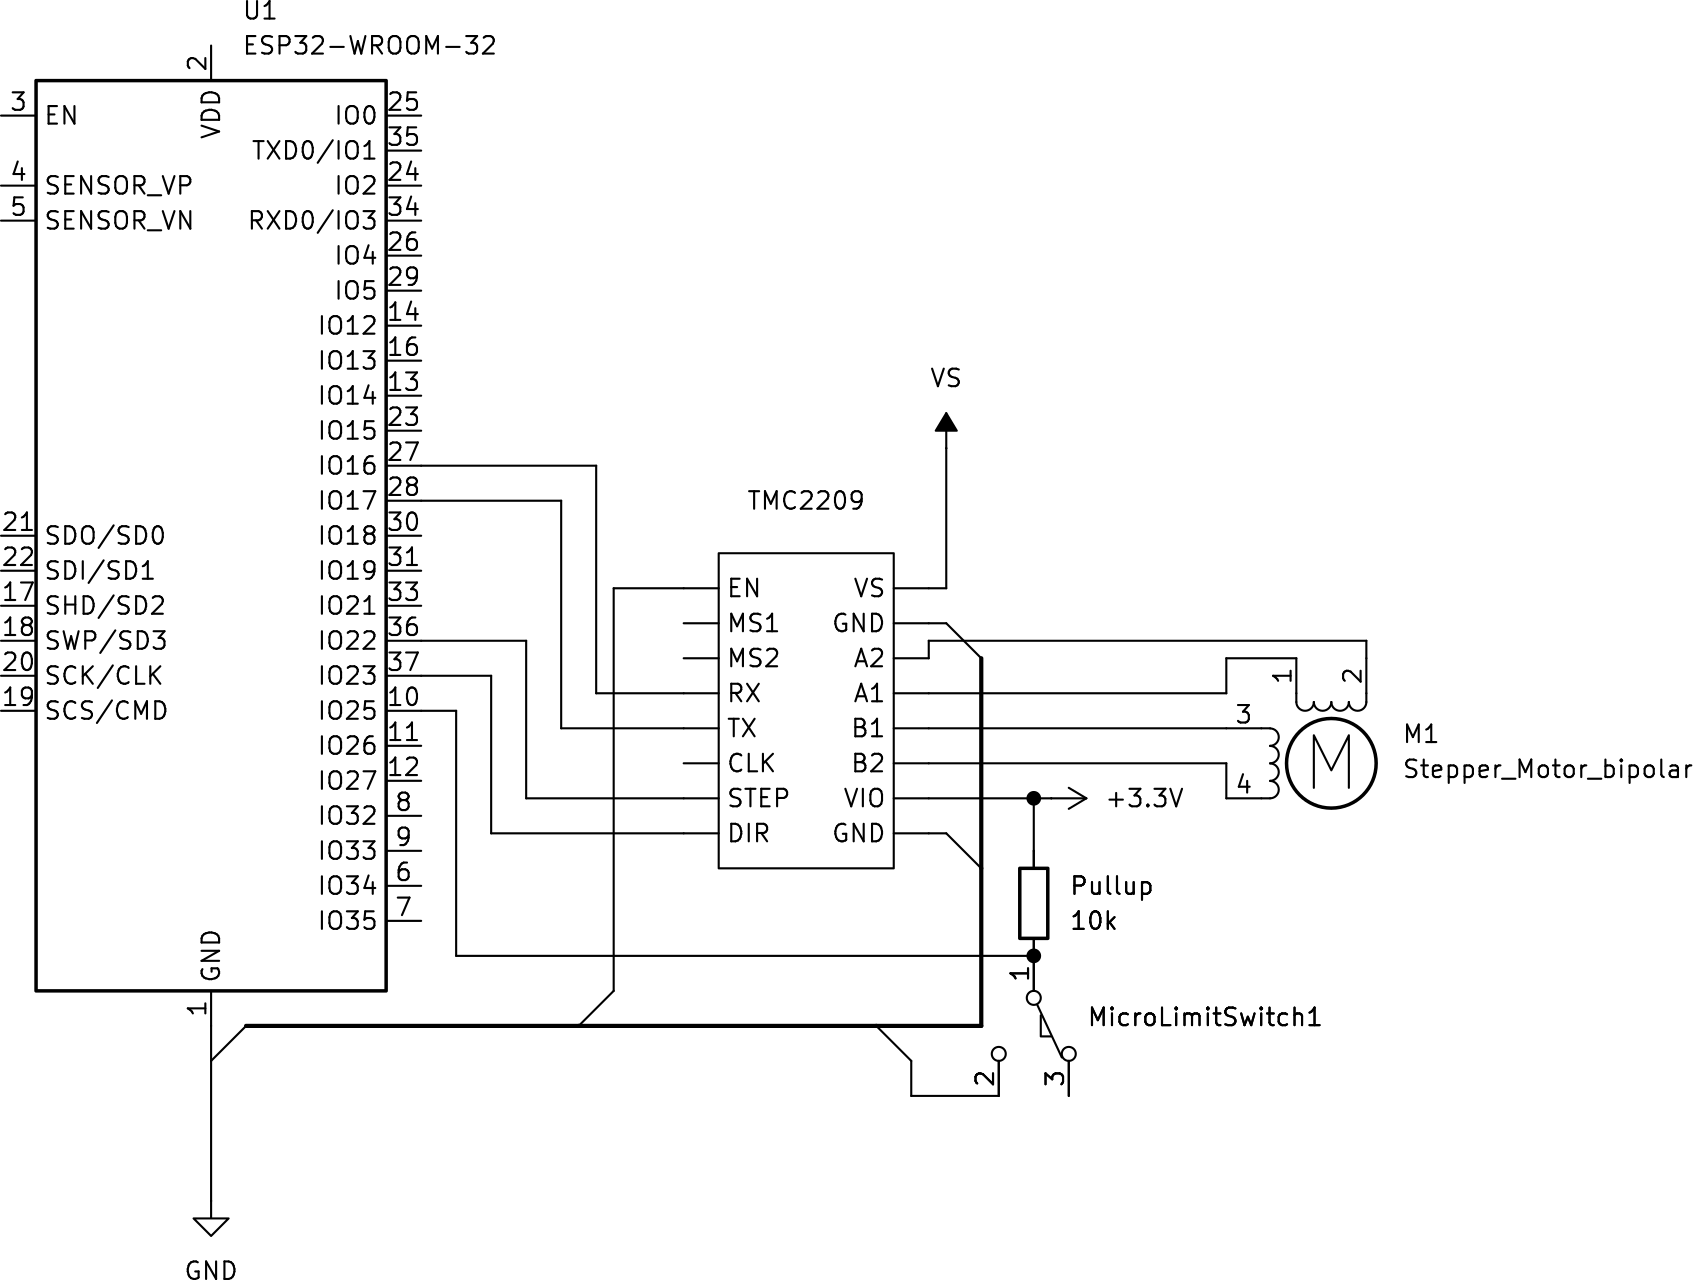
\includegraphics[width=0.75\textwidth]{figures/Wiring_BW.png} 
    \caption{Schematische aansluiting van de elektronische componenten.}\label{fig:schematische_aansluiting} 
\end{figure}


\section{Software ontwerp}
\subsection{Belangrijke functionaliteit in de software}
\begin{itemize}
\item \textbf{Nulzetten}: elke sessie begint met het nulzetten van de pipet via een eindeloopschakelaar.
\item \textbf{Veiligheidsgrenzen}: minimale en maximale volumes worden softwarematig bewaakt.
\item \textbf{Commandostructuur}: eenvoudige commando’s zoals ``A500 R20'' (aspireer 500 $\mu l$ aan 20 $\mu l/s$).
\item \textbf{Logging}: alle acties en fouten worden gelogd.
\end{itemize}
De software is opgebouwd uit drie lagen: de gebruikersinterface, de middleware (robot control API), en de firmware op de ESP32.\ \autoref{fig:Flowchart} toont het overzicht van de communicatie tussen de modules.

\subsection{Opbouw van de software}
De gebruiker start een sequentie via een Python-script, dat via een HTTP- of lokale seriële client de methoden aanroept. Na de methode-aanroep wordt de communicatie via de seriële lijn naar de ESP32 gestuurd, die de motor aanstuurt en een JSON-respons terugstuurt naar de client.


\begin{figure}[H] 
    \centering 
    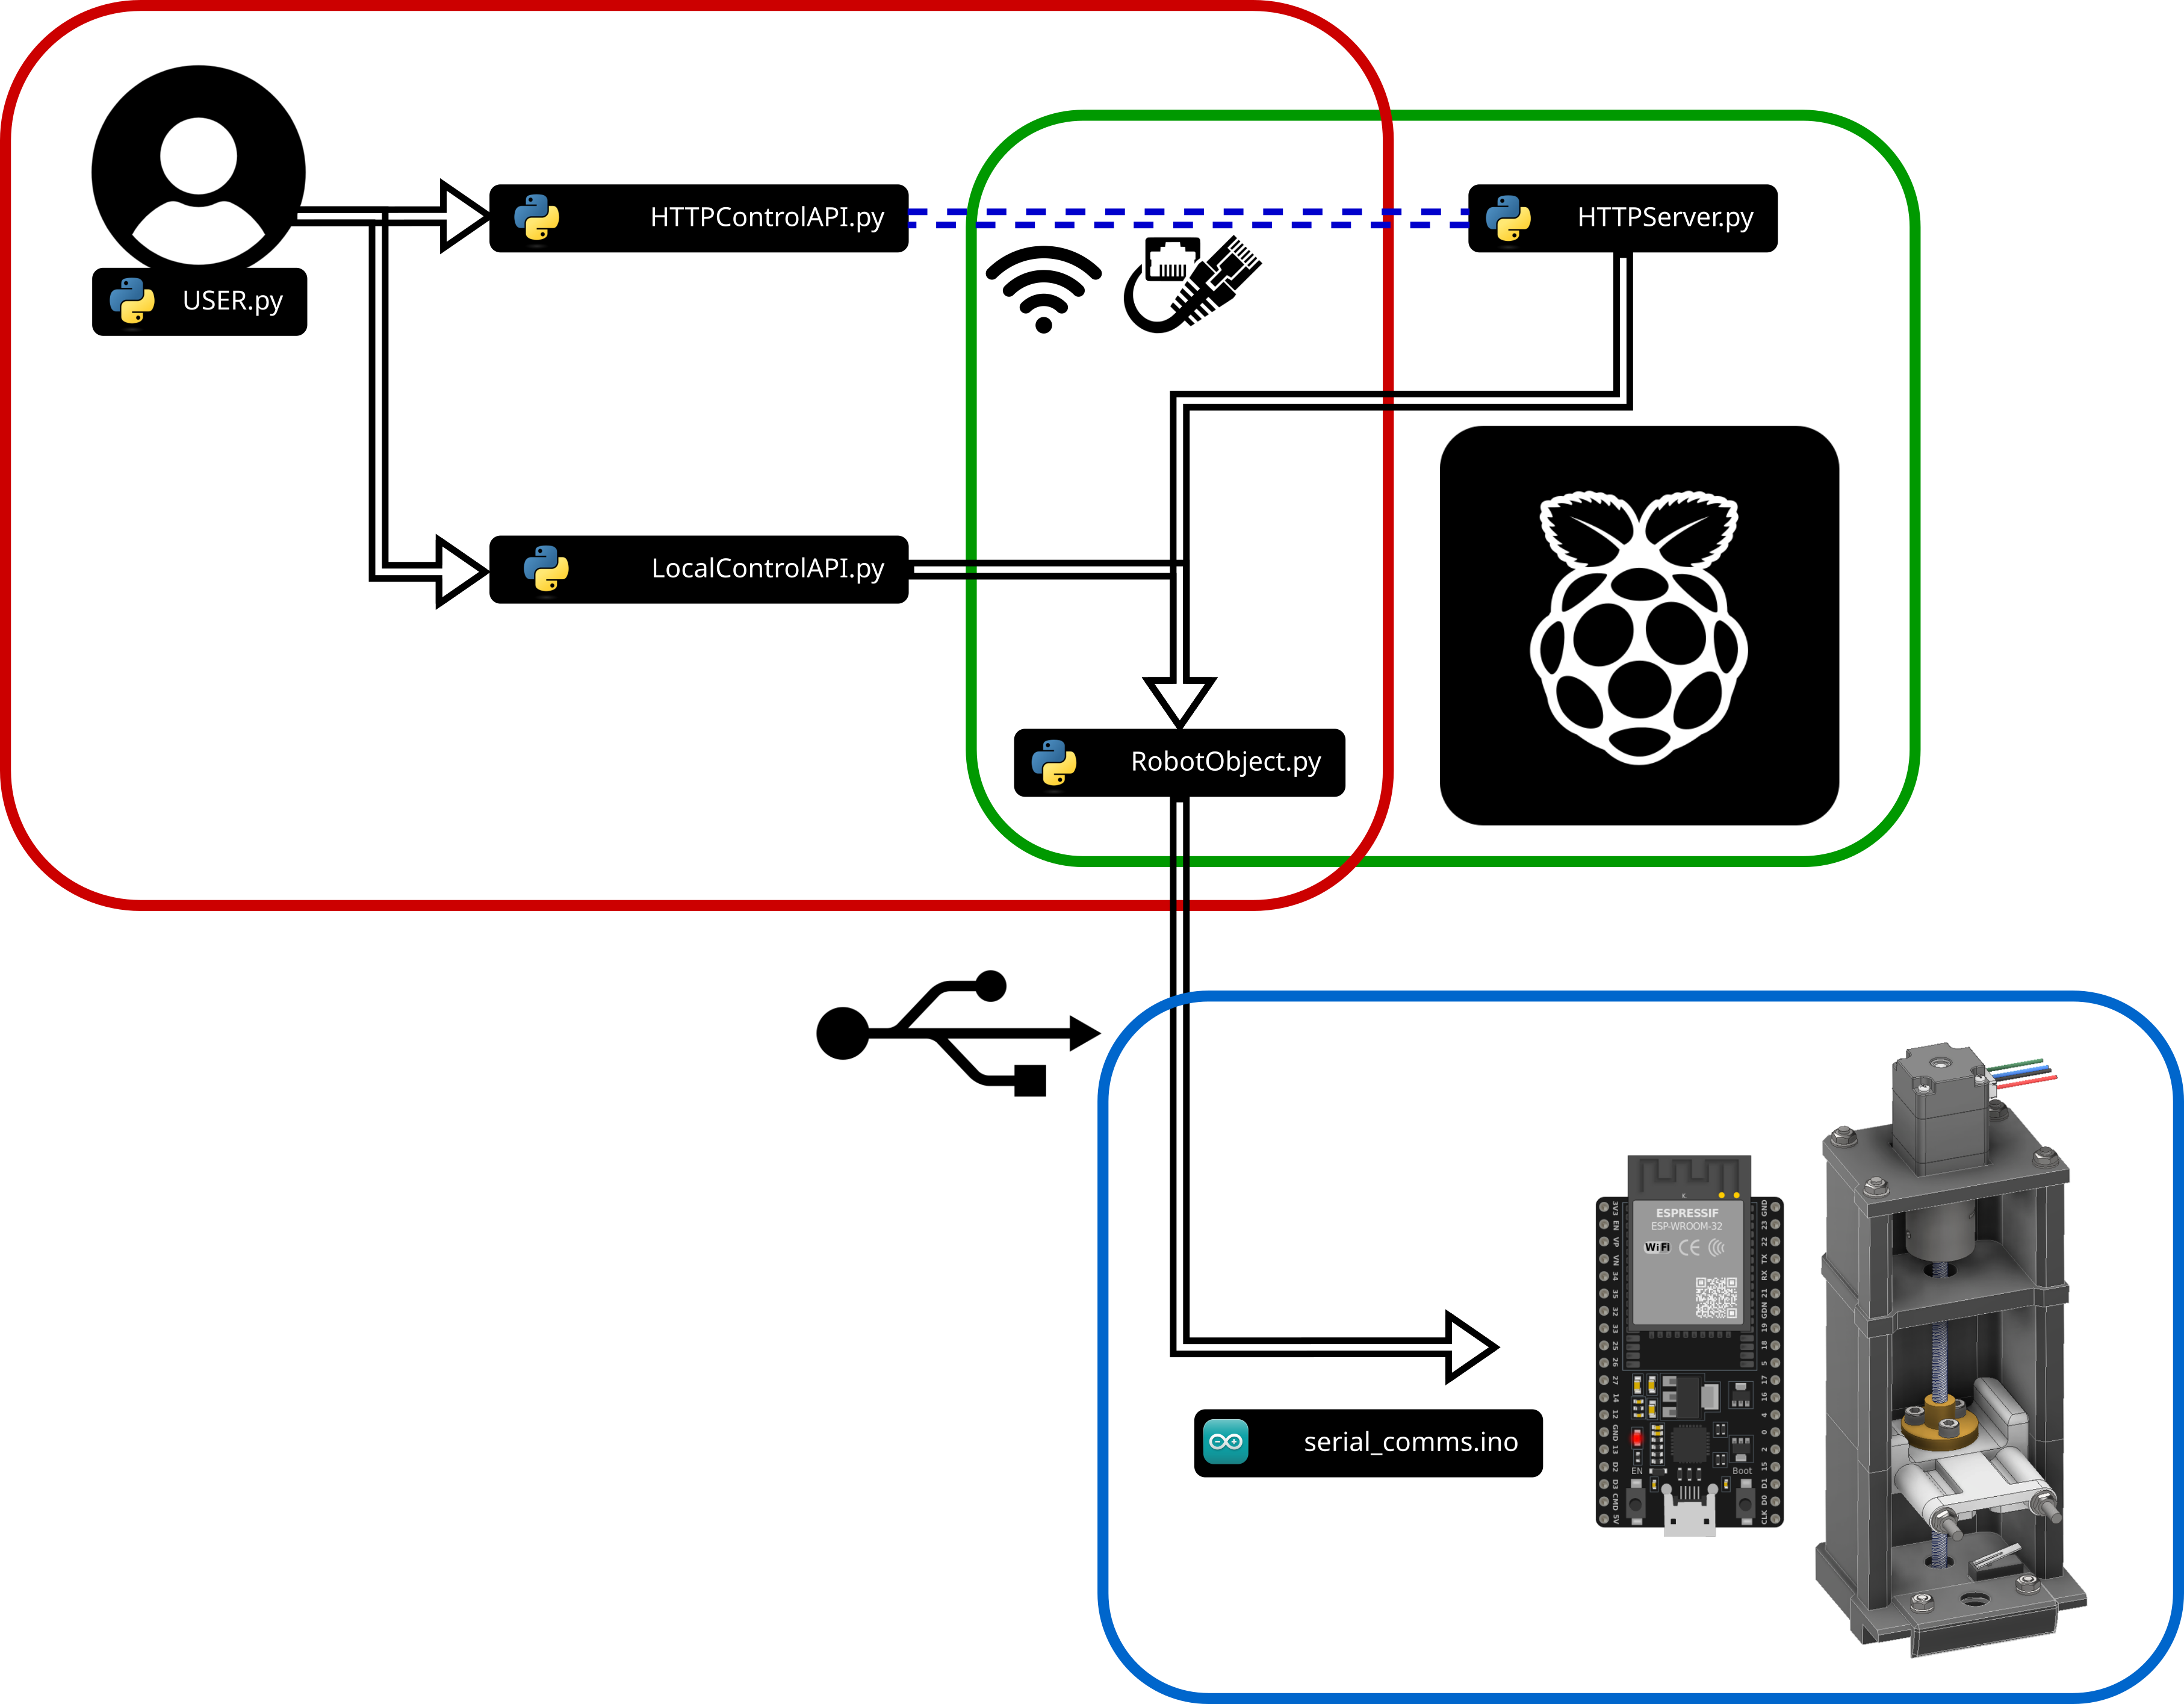
\includegraphics[width=0.75\textwidth]{figures/Flowchart.png} 
    \caption{Overzicht van de softwarearchitectuur en communicatie tussen modules.}\label{fig:Flowchart} 
\end{figure}

